This appendix shows more detailed temperature distributions as referenced in Chapter \ref{scalabilitysim}. 

Shown in Figure \ref{fig:1kW_scalability_detailed}, Figure \ref{fig:10kW_scalability_detailed}, and Figure \ref{fig:100kW_scalability_detailed} are the detailed temperature distributions of the transformers in 1 kW, 10 kW, and 100 kW respectively examined in Chapter \ref{scalabilitysim}. Each transformer is given each individual scale. The results presented in Chapter \ref{scalabilitysim} make it hard to distinguish the detailed temperature distribution for the flatwise-wound transformers due to the large difference in peak winding temperatures as the powers increase. For the flatwise-wound configurations, there is a difference in temperature between the aluminum blocks attached to the dead space and the main ferrite core of the transformers. Given the lower thermal resistance of aluminum compared to ferrite, this observation could be attributed to the stronger cooling condition associated to using a cold plate this time compared to the simulations in Chapter 4. Moreover, the temperature difference is not that significant, with almost negligible at 1 kW operation and around 3$^\circ$C at 100 kW operation. Nevertheless, the thermal management benefit is consistent in all power levels examined.

\begin{figure}[H]
    \centering
    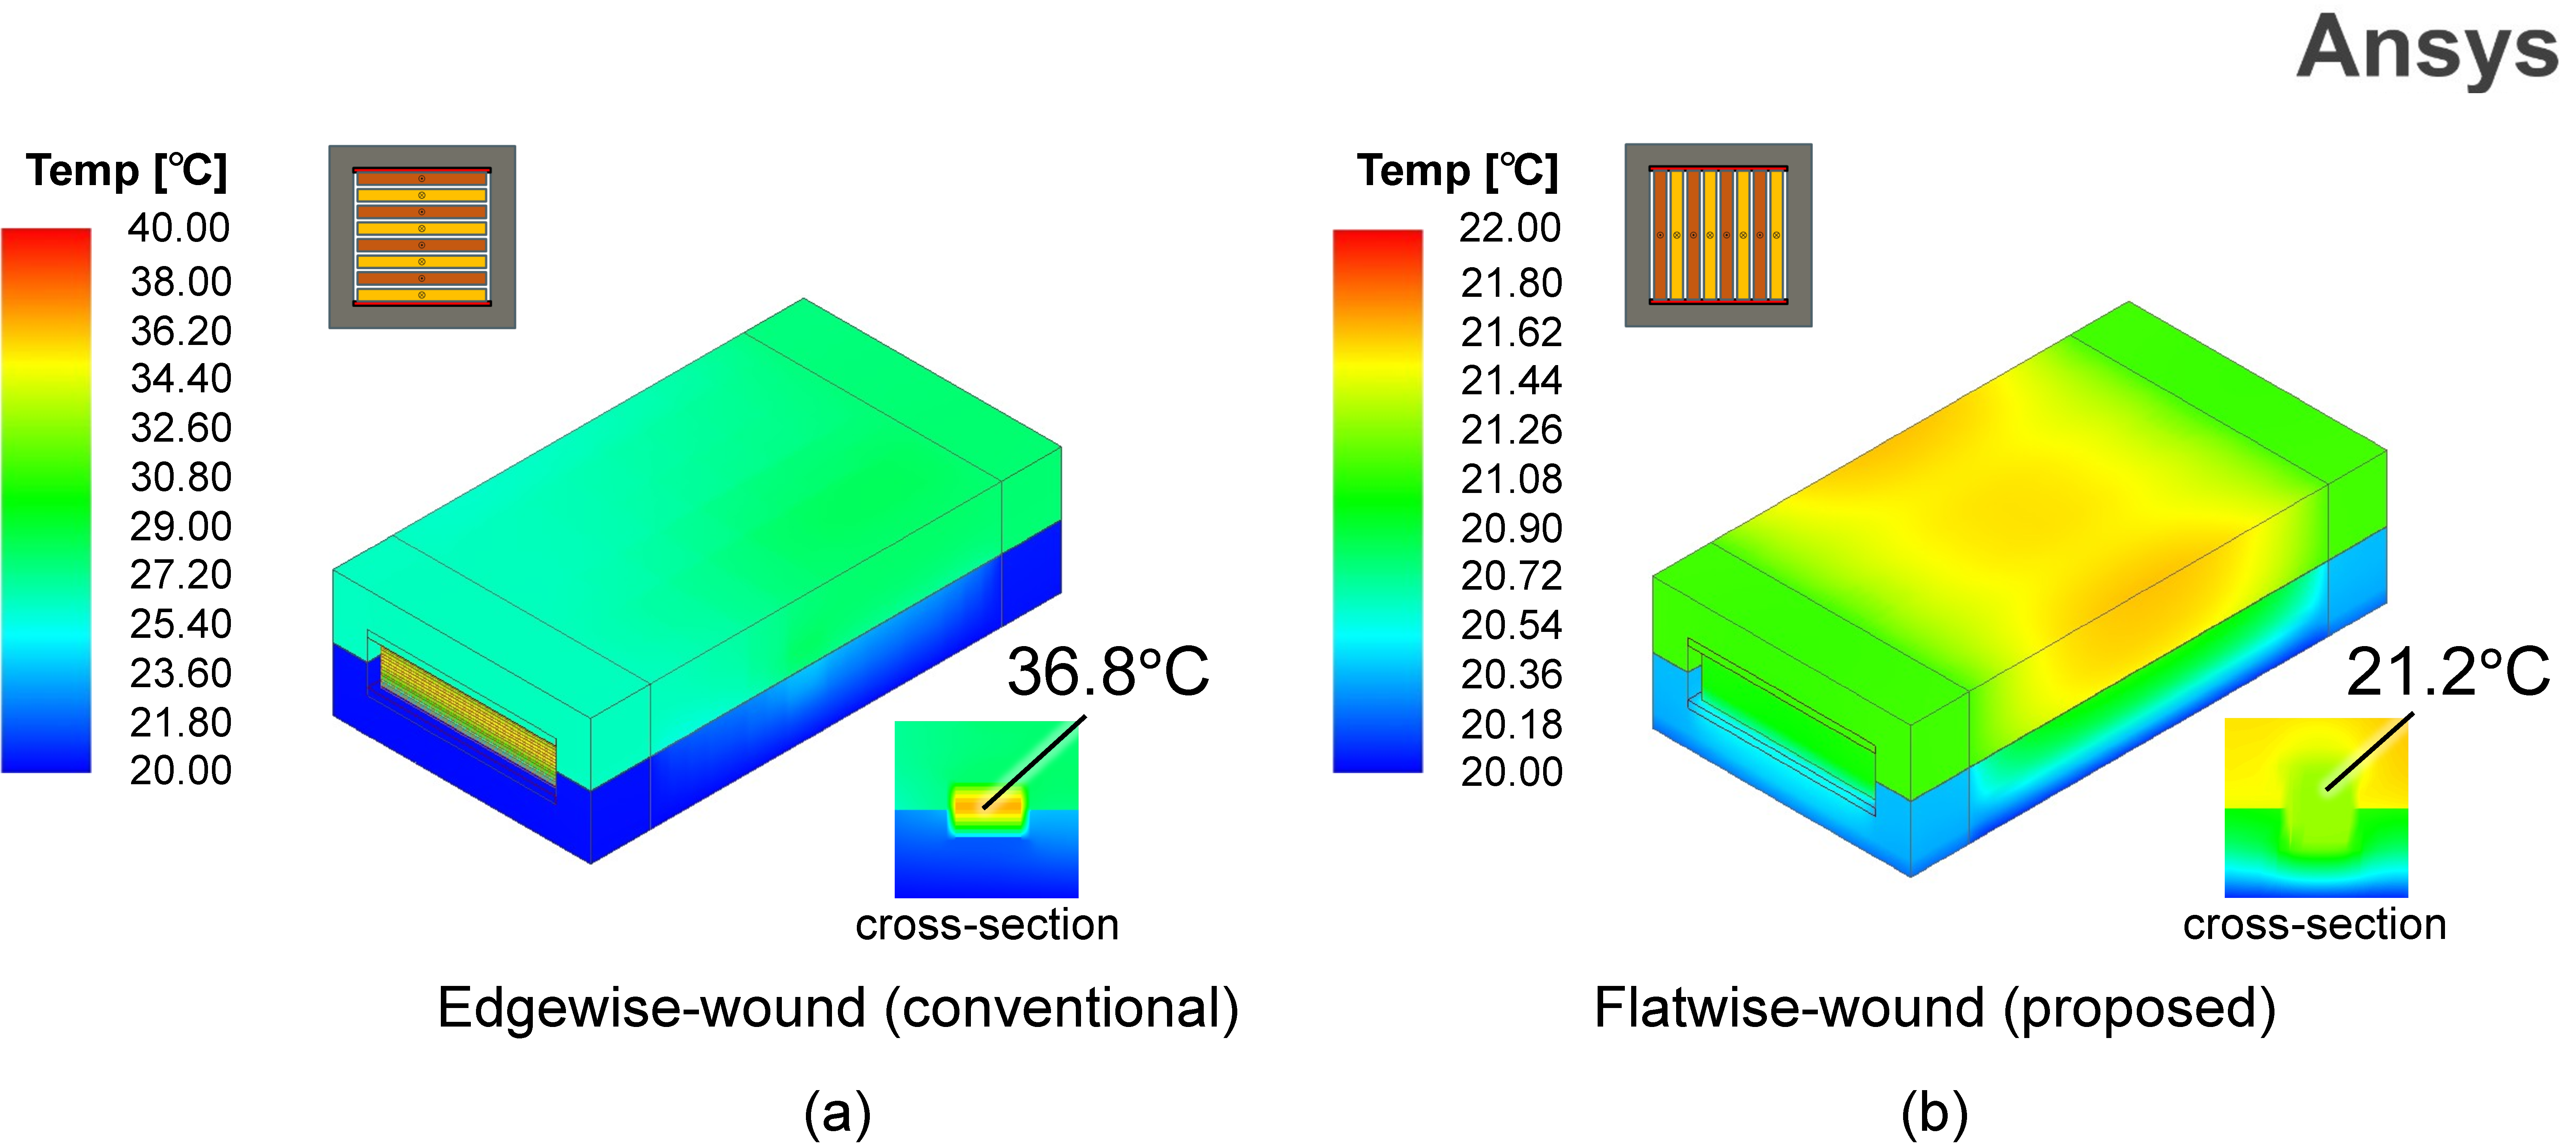
\includegraphics[width=\columnwidth]{images/1kW_scalability_detailed.pdf}
    \caption{Detailed simulated thermal distribution of the evaluated transformer models at 28.5 kHz, 1kW operation with a 20$^\circ$C cold-plate boundary and 25.0$^\circ$C ambient temperature: (a) TrE1, (b) TrF1.}
    \label{fig:1kW_scalability_detailed}
\end{figure}

\begin{figure}[H]
    \centering
    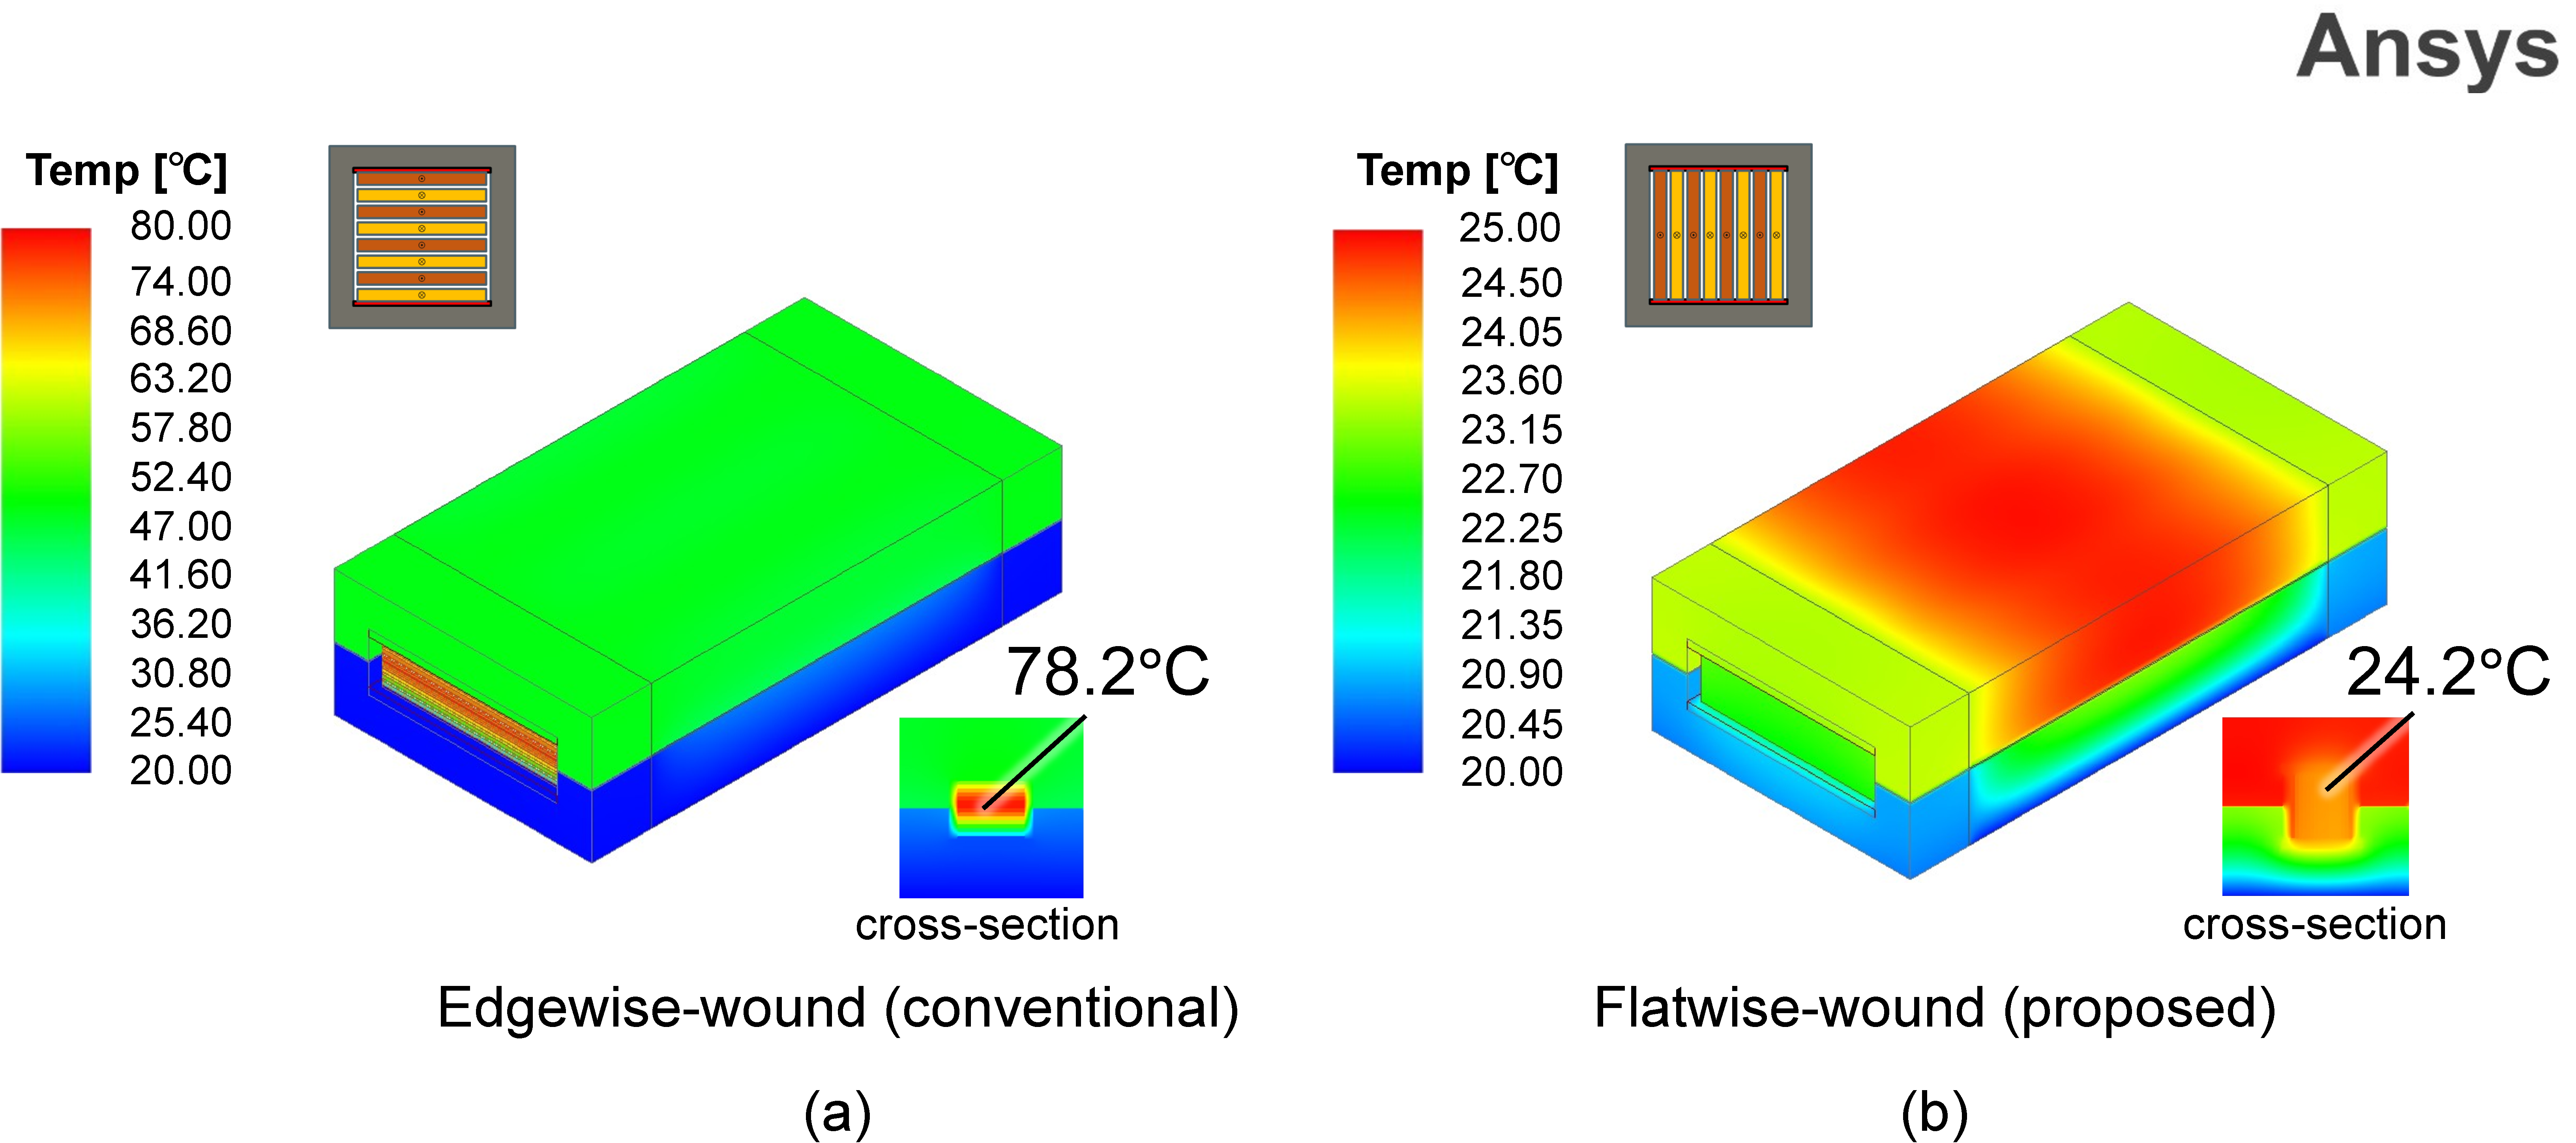
\includegraphics[width=\columnwidth]{images/10kW_scalability_detailed.pdf}
    \caption{Detailed simulated thermal distribution of the evaluated transformer models at 28.5 kHz, 10kW operation with a 20$^\circ$C cold-plate boundary and 25.0$^\circ$C ambient temperature: (a) TrE10, (b) TrF10.}
    \label{fig:10kW_scalability_detailed}
\end{figure}

\begin{figure}[H]
    \centering
    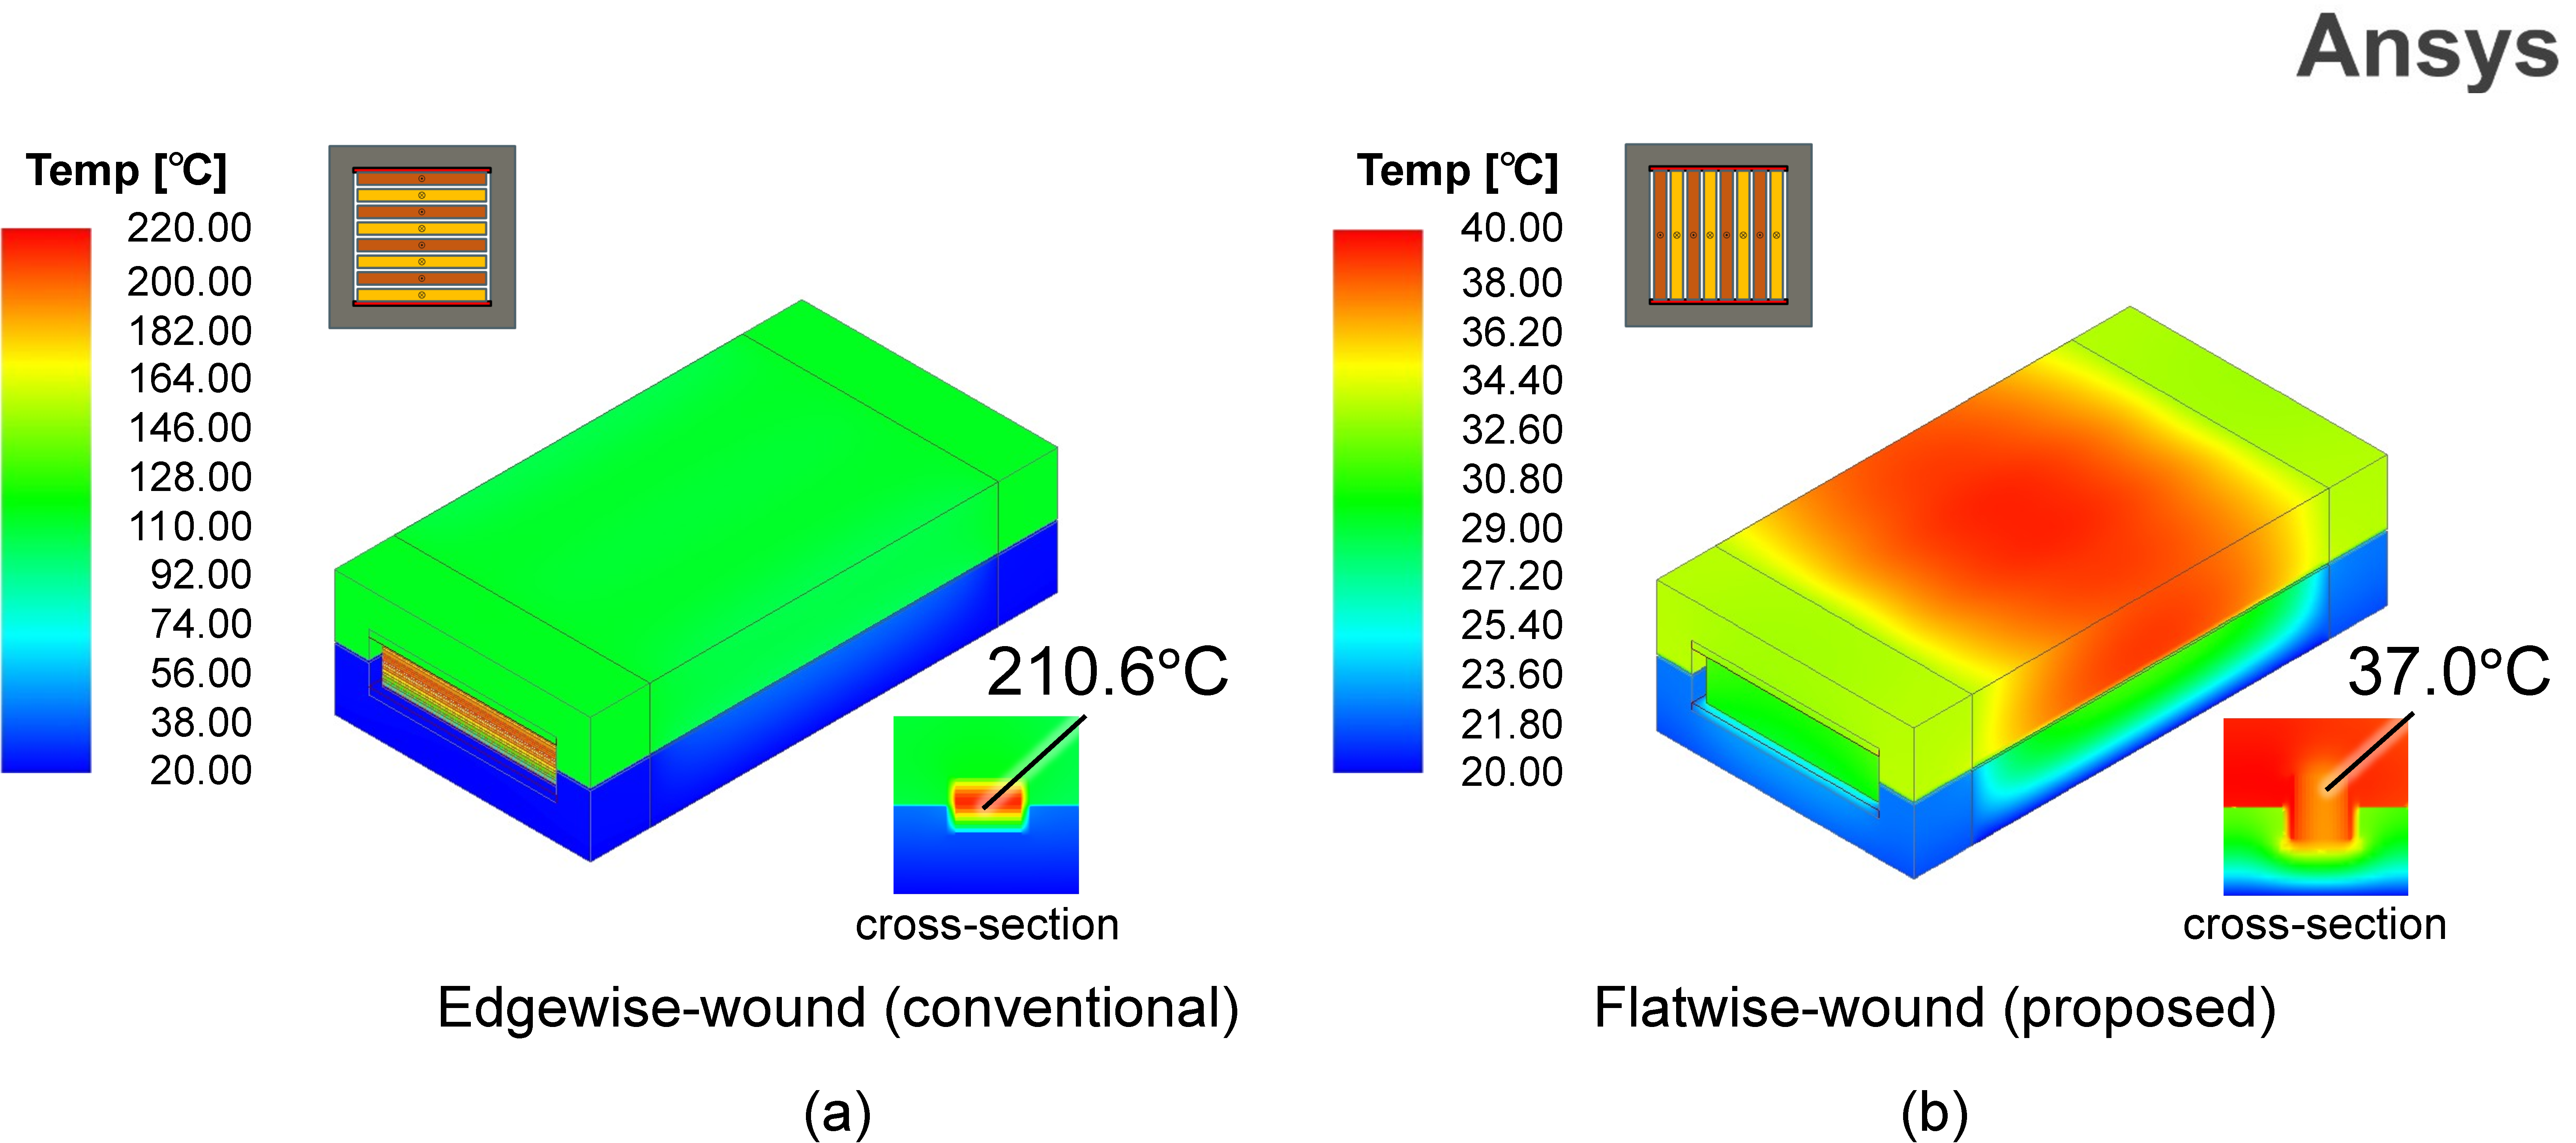
\includegraphics[width=\columnwidth]{images/100kW_scalability_detailed.pdf}
    \caption{Detailed simulated thermal distribution of the evaluated transformer models at 28.5 kHz, 10kW operation with a 20$^\circ$C cold-plate boundary and 25.0$^\circ$C ambient temperature: (a) TrE100, (b) TrF100.}
    \label{fig:100kW_scalability_detailed}
\end{figure}
